\documentclass[11pt]{article}
\usepackage[hidelinks]{hyperref}
\usepackage[letterpaper]{geometry}
\geometry{verbose,tmargin=1in,bmargin=1in,lmargin=1in,rmargin=1in}
\usepackage[acronym,nomain,nonumberlist,nogroupskip,nopostdot]{glossaries} % for glossary of acronyms
\usepackage{siunitx}
\usepackage{verbatim}
\usepackage{booktabs}
\usepackage{multirow}
\usepackage{threeparttable}
\usepackage{longtable}
\usepackage{rotating}
\usepackage{pdflscape}
\usepackage{cancel}
\usepackage{mathrsfs}
\usepackage[mathscr]{euscript}
\usepackage{mhchem}
\setcounter{tocdepth}{4}
\setcounter{secnumdepth}{4}
\usepackage{xcolor}
\usepackage{amsmath,mathtools}
\newcommand{\hO}{\hat{\Omega}}
\newcommand\todo[1]{{\color{red}\bf [TODO: #1]}}
\usepackage{tcolorbox}
\setacronymstyle{long-short}

\newcommand{\mdash}{\discretionary{}{}{\kern 0.1em}---\discretionary{}{}{\kern 0.1em}}
\newcommand\Tstrut{\rule{0pt}{2.6ex}}         % = `top' strut
\newcommand\Bstrut{\rule[-0.9ex]{0pt}{0pt}}   % = `bottom' strut
\newcommand{\beq}{\begin{equation}\begin{aligned}}
\newcommand{\eeq}{\end{aligned}\end{equation}}
\newcommand{\beqs}{\begin{equation*}\begin{aligned}}
\newcommand{\eeqs}{\end{aligned}\end{equation*}}
\newcommand{\ans}[1]{{\color{violet}#1}}
\newcommand{\volume}{\mathop{\ooalign{\hfil$V$\hfil\cr\kern0.08em--\hfil\cr}}\nolimits} % Cursed workaround for typsetting control volume LOL
\newcommand{\Nc}{\mathscr{N}}
\newcommand{\ddt}{\frac{\partial}{\partial t}}

\setlength{\parskip}{5pt}

\begin{document}
\noindent {\bf \Large NPRE 455: Homework 4}\\

\begin{tcolorbox}
On this homework, you will perform your first solutions of the neutron diffusion equation. For the remainder of the course, unless you are explicitly told what vacuum boundary condition to use, the choice is yours (extrapolated vs. Robin).
\end{tcolorbox}
\vspace{2cm}

\noindent 1. ({\bf factual concept recall}) Provide a {\it short} (1-2 sentences) answer to each of the following questions.

\begin{itemize}
\item[(a)] ({\bf 2 points}) The total interaction term in the neutron transport equation is $\Sigma_t(\vec{r},E,t,\hO)\psi(\vec{r},E,t,\hO)$. Why is the total interaction term given by $\Sigma_a(\vec{r},t)\phi(\vec{r},t)$ in the one-speed diffusion equation? (In other words, why use $\Sigma_a$ instead of $\Sigma_t$)?
\item[] \ans{The total section comprises both absorption and scattering, but scattering doesn't remove a neutron from the system, only changing its energy.
If all neutrons are simplified to one energy group, then scattering doesn't remove any of them and is essentially ignorable w.r.t total interaction.}
\item[(b)] ({\bf 1 point}) When can the $-\nabla\cdot (D\nabla\phi)$ term be written as $-D\nabla^2\phi$?
\item[] \ans{If the diffusion constant $D$ does not change with respect to position, such as in a uniform material, then it can be separated and applied to the left of the $\nabla$ operator this way.}
\item[(c)] ({\bf 2 points}) What is the difference between a distributed and localized source? Give an example of each.
\item[] \ans{In a distributed source, like spontaneous fission of $^{252}$Cf distributed in the fuel or lithium/beryllium struck by alpha particles (not neutrons so it's not flux-based), the source is considered volumetrically at every point, and shows up in the balance equation. In a localized source, like an idealized painted coating of $^{252}$Cf on a sphere, the volume doesn't have to be considered in a new diffusion equation and can instead be treated as a modified boundary condition.}
\item[(d)] ({\bf 2 points}) Explain the extrapolated vacuum boundary condition. Does it mean that the flux decreases linearly in the vacuum region?
\item[] \ans{In the extrapolated flux vacuum boundary condition, we linearly extrapolate the flux and its gradient to some distance $d=2.1312D$ away where it will reach 0. This does \emph{not} mean that the flux actually decreases linearly until that point, rather just that this provides a good approximate constraint to apply.}
\item[(e)] ({\bf 2 points}) Give a physical interpretation for $L$, the neutron diffusion length. How is it different from the mean free path, which has the same units as $L$?
\item[] \ans{Physically, $L$ corresponds to half of the straight-line distance between source to absorption, averaging over when it scatters and changes direction, whereas the mean free path is the distance between \emph{any} interaction, including scattering.}
\item[(f)] ({\bf 1 point}) What is a typical value of $L$ in a Pressurized Water Reactor (PWR) and Sodium Fast Reactor (SFR)?
\item[] \ans{A typical PWR might have an $L$ of 5.91~cm, whereas an SFR would typically have a much higher $L$ around 23.61~cm.}
\end{itemize}

\clearpage
\noindent 2. ({\bf diffusion balance equation}) Consider a spherical shell between $r$ and $r+dr$. Neutrons enter and leave the shell by streaming, and are produced and lost within the shell due to fission and absorption, respectively.

\begin{figure}[htb!]
\centering
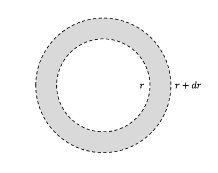
\includegraphics[width=0.3\linewidth]{figures/hw4Q_spherical_shell.png}
\end{figure}

\begin{enumerate}
\item[(a)] ({\bf 10 points}) Derive the one-group, steady-state, 1-D ($r$-only) neutron balance equation in spherical geometry. Follow the approach used in class to derive the balance equation for the Cartesian cases. ({\it Hint}: Unlike the Cartesian case, the area for the neutron current calculation on the two surfaces will be different).
\item[] \ans{
    If we consider the given control volume, and neutrons are conserved, then over that control volume the change in neutrons over time should be equivalent to the source rate minus the loss rate:
    \begin{gather*}
        \mathrm{time~rate~of~change=sources-losses}\\
        \mathrm{sources=fission~rate+current~entering+delayed+external}\\
        \mathrm{losses=absorption~rate+current~leaving}
    \end{gather*}

    Rather than a differential volume with respect to radius and solid angle $ r^2\sin(\varphi)d r d\theta d\varphi$, we consider this shell, already integrated around solid angle, only differential to radius, $4\pi r^2d r$.\\
    Assuming properties and flux are uniform across solid angle, the overall time rate of change, fission rate, delayed and external sources, and absorption rate can all be considered relative to this differential shell:
    \begin{equation*}
        \ddt(n)4\pi r^2d r = \left((\nu_p\Sigma_f-\Sigma_a)\phi + s + \sum_{i=1}^{N}\lambda_iC_i\right)4\pi r^2d r + \mathrm{current~in-current~out}
    \end{equation*}
    Given that we consider the whole shell, the only two surfaces we need to consider are the inner and outer surfaces of the shell.
    Additionally, let us combine the current entering and the current leaving into simply the net current entering each surface:
    % \begin{equation}
    %     \mathrm{net~current}=\vec{J}(r)\cdot\hat{n(r)}4\pi r^2d r+\vec{J}(r+dr)\cdot\hat{n(r+dr)}4\pi (r+dr)^2d r
    % \end{equation}
    \begin{align*}
        \mathrm{net~current}&=J(r)4\pi r^2-J(r+dr)4\pi (r+dr)^2\\
        &=-4\pi d(r^2J)
    \end{align*}
    where $J(r)$ is the current in the outwards $\hat{r}$ direction, since we assume current is negligible in the angular directions. (If the net current were \emph{inwards}, this net equation would still hold, resulting in neutrons instead leaving at $r$ and entering at $r+dr$)\\

    Plugging back into our balance and dividing both sides by $4\pi r^2dr$:
    \begin{align*}
        \ddt(n)4\pi r^2d r &= \left((\nu_p\Sigma_f-\Sigma_a)\phi + s + \sum_{i=1}^{N}\lambda_iC_i\right)4\pi r^2d r-4\pi d(r^2J) \\
        \ddt(n)&= (\nu_p\Sigma_f-\Sigma_a)\phi + s + \sum_{i=1}^{N}\lambda_iC_i    - \frac{1}{r^2}\frac{d(r^2J)}{dr} \\
    \end{align*}
    Finally, applying a diffusive current assumption $\vec{J}=-\nabla\phi$, and that in our angularly symmetric spherical coordinates, the gradient of flux is $\nabla\phi=\frac{\partial\phi}{\partial r}$:
    \begin{align*}
        \ddt(n)&= (\nu_p\Sigma_f-\Sigma_a)\phi + s + \sum_{i=1}^{N}\lambda_iC_i    - \frac{1}{r^2}\frac{d(r^2J)}{dr} \\
        \ddt(n)&= (\nu_p\Sigma_f-\Sigma_a)\phi + s + \sum_{i=1}^{N}\lambda_iC_i    - \frac{1}{r^2}\frac{d}{dr}\left(-r^2 D \frac{\partial\phi}{\partial r}\right) \\
        \ddt(n)- \frac{1}{r^2}\frac{d}{dr}\left(r^2 D \frac{\partial\phi}{\partial r}\right)&= (\nu_p\Sigma_f-\Sigma_a)\phi + s + \sum_{i=1}^{N}\lambda_iC_i \\
    \end{align*}
    \begin{equation*}
        \boxed{\frac{1}{v}\frac{\partial\phi}{\partial t}- \frac{1}{r^2}\frac{d}{dr}\left(r^2 D \frac{\partial\phi}{\partial r}\right)= (\nu_p\Sigma_f-\Sigma_a)\phi + s + \sum_{i=1}^{N}\lambda_iC_i}
    \end{equation*}
    Or, in steady state:
    \begin{equation*}
        \boxed{- \frac{1}{r^2}\frac{d}{dr}\left(r^2 D \frac{\partial\phi}{\partial r}\right)= (\nu_p\Sigma_f-\Sigma_a)\phi + s + \sum_{i=1}^{N}\lambda_iC_i}
    \end{equation*}
    % The time rate of change of the volume can be formulated by integrating the local time rate of change over every point in the volume:
    % \begin{gather*}
    %     \mathrm{time~rate}=\ddt\int d\volume\Nc(\vec{r},t) \\
    %     = \int d\volume \ddt\Nc(\vec{r},t)\\
    %     = \int_{0}^{\pi}\int_{0}^{2\pi}\int_{r}^{r+dr}\Nc(\vec{r},t)\rho^2\sin(\varphi)d\rho d\theta d\varphi
    % \end{gather*}
    % While this shows evaluation of that volume integral in spherical coordinates, for the moment the integral will be left as $\int d\volume$.\\
    % Parts of both sources and losses will be proportional to flux: absorption and fission. These will be found by integrating the reaction rate $\Sigma_{i\in\{a,f\}}\phi(\vec{r},t)$ across the control volume.\\
    % For fission:

}
\end{enumerate}



\clearpage
\noindent 3. ({\bf diffusion boundary conditions}) Write down (but do not solve!) the boundary conditions for the following multi-region, 1-D problems. If there are any vacuum boundaries, give two options for the boundary condition -- the extrapolated condition as well as the Robin condition.

\begin{enumerate}
\item[(a)] ({\bf 6 points}) See Fig. \ref{fig:3a}. Region 2 has a distributed source of strength $S$ [neutrons/cm$^3$/s].


\begin{figure}[htb!]
\centering
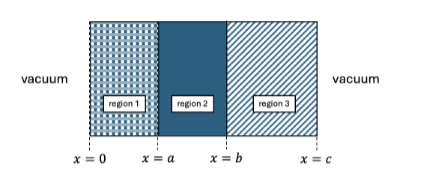
\includegraphics[width=0.6\linewidth]{figures/hw4Q_3dr.png}
\caption{Cartesian domain}
\label{fig:3a}
\end{figure}
\item[] \ans{
    Since we have three regions, each with their own diffusion equation (2 derivatives), we should look for a total of 6 boundary conditions.\\

    For the two material boundaries at $x=a$ and $x=b$, we can assume continuous flux:
    \begin{align}
        \phi_1(x=a)&=\phi_2(x=a) \\
        \phi_2(x=b)&=\phi_3(x=b)
    \end{align} 
    where $\phi_i$ represents the flux in region $i$.
    We also know that neutrons are conserved, so we can apply the jump condition without any neutron source:
    \begin{align*}
        \left.\vec{J_1}\cdot\hat{n}\right|_{x=a}&=\left.\vec{J_2}\cdot\hat{n}\right|_{x=a}\\
        \left.-D_1\frac{d\phi_1}{dx}\right|_{x=a}&=\left.-D_2\frac{d\phi_2}{dx}\right|_{x=a}
    \end{align*}
    \begin{align}
        -D_1\frac{d\phi_1}{dx}(x=a)&=-D_2\frac{d\phi_2}{dx}(x=a)\\
        -D_2\frac{d\phi_2}{dx}(x=b)&=-D_3\frac{d\phi_3}{dx}(x=b)
    \end{align}

    Finally, for the fifth and sixth boundary conditions, we can consider the vacuum boundaries at $x=0$ and $x=c$.
    We could consider the extrapolated condition at a distance $2.1312D$ away:
    \begin{align*}
        \phi_1(x=-2.1312D)&=0\\
        \phi_3(x=c+2.1312D)&=0
    \end{align*}
    Alternatively, we could consider the more explicit condition that inward current $J_{-}=\frac{\phi}{4}+\frac{1}{2}D\nabla\phi\cdot\hat{n}$ is zero:
    \begin{align*}
        J_{-}=0&=\frac{\phi}{4}+\frac{1}{2}D\nabla\phi\cdot\hat{n}\\
        &=\frac{\phi}{4}+\frac{1}{2}D\frac{d\phi}{dx}\hat{n}_x(x)
    \end{align*}
    Applying to the left edge at $x=0$ where $\hat{n}_x=-1$ and the right edge at $x=c$ where $\hat{n}_x=1$,
    \begin{align}
        \frac{\phi_1(x=0)}{4}-\frac{1}{2}D_1\frac{d\phi_1}{dx}(x=0)&=0\\
        \frac{\phi_3(x=c)}{4}+\frac{1}{2}D_3\frac{d\phi_3}{dx}(x=c)&=0
    \end{align}
}

\item[(b)] ({\bf 4 points}) See Fig. \ref{fig:3b}. Material 2 continues to $\pm\infty$ on both sides.

\begin{figure}[htb!]
\centering
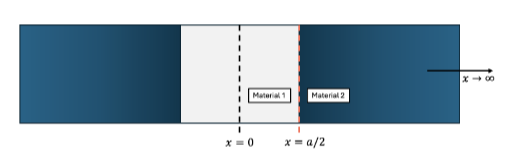
\includegraphics[width=0.8\linewidth]{figures/hw4Q_2dregion.png}
\caption{Cartesian domain}
\label{fig:3b}
\end{figure}

\item[] \ans{
    Let us consider the system symmetric around the plane $x=0$.
    We can now consider one set of solutions for $0\leq x<\infty$.
    This yields two solution regions, requiring four boundary conditions.\\

    At $x=0$, we apply a symmetry condition with no localized source on the plane:
    \begin{align*}
        J_+(0_-)&=J_+(0_+)\\
        \frac{\phi_1(x=0_-)}{4}-\frac{1}{2}D_1\frac{d\phi_1}{dx}(x=0_-)&=\frac{\phi_1(x=0_+)}{4}+\frac{1}{2}D_1\frac{d\phi_1}{dx}(x=0_+)\\
        \frac{d\phi_1}{dx}(x=0)&=0
    \end{align*}

    For the boundary between materials 1 and 2, let us again consider continuity of flux and the continuity of current crossing the boundary:
    \begin{align*}
        \phi_1(x=\frac{a}{2})&=\phi_2(x=\frac{a}{2})\\
        -D_1\frac{d\phi_1}{dx}(x=\frac{a}{2})&=-D_2\frac{d\phi_2}{dx}(x=\frac{a}{2})
    \end{align*}
    And finally let us constrain that as $x\rightarrow\infty$, the flux is either 0 or finite:
    \begin{equation*}
        \phi_2(x\rightarrow\infty)=0\mathrm{~or~finite}
    \end{equation*}
}

\item[(c)] ({\bf 4 points}) See Fig. \ref{fig:3c}. The red curve indicates a source of neutrons of strength $S$ [neutrons/cm$^2$/s] coated on the interface.

\begin{figure}[htb!]
\centering
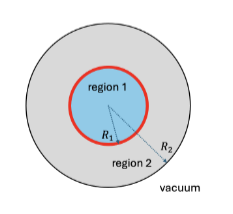
\includegraphics[width=0.3\linewidth]{figures/hw4Q_sphere_r.png}
\caption{Spherical domain}
\label{fig:3c}
\end{figure}

\item[] \ans{
    Once again we have two regions, requiring four boundary conditions.\\
    Given radial symmetry around the origin, and the lack of a point source, the symmetry condition at $r=0$ simplifies to requiring no net current at the origin:
    \begin{equation}
        -D_1\frac{d\phi_1}{dr}(0)=0
    \end{equation}
    At the boundary between regions 1 and 2, even with the localized source, we still require continuity of flux:
    \begin{equation}
        \phi_1(r=R_1)=\phi_2(r=R_1)
    \end{equation}
    and a jump condition (conservation of current crossing boundaries, including the neutrons generated at the boundary):
    \begin{equation}
        \lim_{r\rightarrow R_1}\left[-D_2\frac{d\phi_2(r)}{dr}+D_1\frac{d\phi_1(r)}{dr}\right]=S
    \end{equation}
    Finally, at the vacuum, we may either consider an extrapolated boundary a distance $2.1312D$ away:
    \begin{equation*}
        \phi_2(r=R_2+2.1312D)=0
    \end{equation*}
    or the more explicit condition of no incoming current at $R_2$:
    \begin{equation}
        J_{-,2}=\frac{\phi_2(R_2)}{4}+\frac{D}{2}\frac{d\phi_2(R_2)}{dr}=0
    \end{equation}
}

\end{enumerate}



\clearpage
\noindent 4. ({\bf non-multiplying flux solution}) A point source emitting $S$ neutrons/s is placed at the center of a non-multiplying sphere with radius $R$\ans{, as shown in Figure~\ref{fig:p4sphere}}.
% add question about value of current being so small - does it make sense depending on L?
\begin{figure}[!htb]
    \centering
    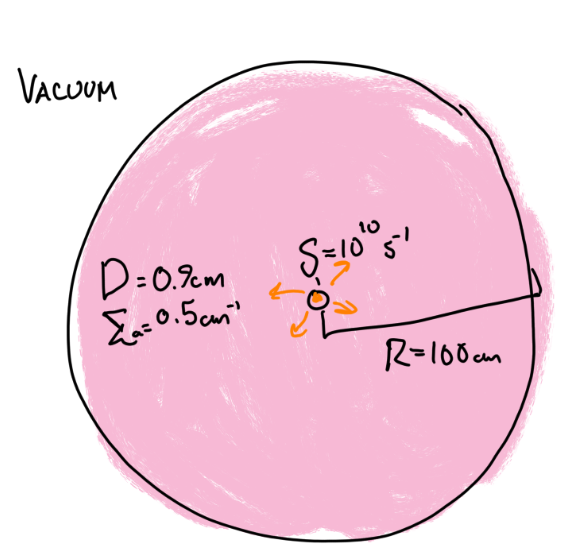
\includegraphics[width=0.7\linewidth]{figures/hw4_p4sphere.png}
    \caption{A point source of strength $S$ lying at the center of a non multiplying sphere of radius $R$.}
    \label{fig:p4sphere}
\end{figure}
\begin{enumerate}
\item[(a)] ({\bf 8 points}) Show that the flux in the sphere is given by the following. Use an extrapolated vacuum boundary condition. ({\it Hint}: to obtain the given solution form, recall the identity: $A\sinh{bx}+B\cosh{bx}=C\sinh{\left\lbrack b(a-x)\right\rbrack}$).

\beq
\label{eq:phi1}
\phi(r)=\frac{S}{4\pi D\sinh{\frac{\tilde{R}}{L}}}\frac{\sinh{\frac{\tilde{R}-r}{L}}}{r}
\eeq
\item[] \ans{
    Let us start with the general neutron diffusion equation:
    \begin{equation}
        \ddt\phi-\nabla D\nabla\phi = (\nu_p\Sigma_f - \Sigma_a)\phi + s + \sum_{i=1}^{N}\lambda_iC_i
    \end{equation}
    Then simplifying to 1D spherical coordinates, with uniform properties, in steady-state operation, without multiplication or a distributed source:
    \begin{align*}
    -\nabla D\nabla\phi &= - \Sigma_a\phi\\
    \frac{1}{r^2}\frac{d}{dr}\left(r^2 \frac{\partial\phi}{\partial r}\right) - \frac{\Sigma_a}{D}\phi&=0\\
    \frac{1}{r^2}\frac{d}{dr}\left(r^2 \frac{\partial\phi}{\partial r}\right) - \frac{1}{L^2}\phi&=0\\
    \end{align*}
    where $L=\sqrt{\frac{D}{\Sigma_a}}$.
    Applying the substitution $\phi(r)=\mu(r)/r$:
    \begin{align*}
        \frac{1}{r^2}\left\lbrack \frac{d}{dr}\left(r^2\frac{d\phi(r)}{dr}\right) \right\rbrack &-\frac{1}{L^2}\phi(r)=0 \\  
        \frac{1}{r^2}\left\lbrack \frac{d}{dr}\left(r^2\frac{d}{dr}\left[\frac{\mu(r)}{r}\right]\right) \right\rbrack &-\frac{1}{L^2}\left(\frac{\mu(r)}{r}\right)=0 \\
        \frac{1}{r^2}\left\lbrack \frac{d}{dr}\left(r^2\left[\frac{\mu'(r)r - \mu(r)}{r^2}\right]\right) \right\rbrack &-\frac{1}{L^2}\left(\frac{\mu(r)}{r}\right)=0 \\
        \frac{1}{r^2}\left\lbrack \frac{d}{dr}\left(\mu'(r)r - \mu(r)\right) \right\rbrack &-\frac{1}{L^2}\left(\frac{\mu(r)}{r}\right)=0 \\
        \frac{1}{r^2}\left\lbrack \mu''(r)r + \mu'(r) - \mu'(r) \right\rbrack &-\frac{1}{L^2}\left(\frac{\mu(r)}{r}\right)=0 \\
        \frac{\mu''(r)}{r} &-\frac{1}{L^2}\left(\frac{\mu(r)}{r}\right)=0 \\
        \mu''(r) &-\frac{1}{L^2}\mu(r) = 0
    \end{align*}
    We can apply the Helmholtz solution for hyperbolic trigonometry functions, and revert our earlier substitution:
    \begin{align*}
        \mu(r)&=A\sinh(r/L)+B\cosh(r/L)\\
        \frac{\mu(r)}{r}=\phi(r)&=\frac{A\sinh(r/L)}{r}+\frac{B\cosh(r/L)}{r}
    \end{align*}
    Allow us to make the following substitution:
    \begin{equation*}
        \frac{A\sinh(r/L)}{r}+\frac{B\cosh(r/L)}{r}=\phi(r)=\frac{C}{r}\sinh\left[(a-r)/L\right]
    \end{equation*}
    Now, using the extrapolated vacuum boundary condition, for an extrapolated boundary $\tilde{R}=R+\tilde{a}$:
    \begin{align*}
        \phi(\tilde{R})=0&=\frac{C}{\tilde{R}}\sinh\left[(a-\tilde{R})/L\right]\\
        &\color{gray}\rightarrow a=\tilde{R}
    \end{align*}
    And finally applying a symmetric condition around the source at $r=0$:
    \begin{gather*}
        \lim_{r\rightarrow0}\left[-D\frac{d\phi(r)}{dr}=\frac{S}{4\pi r^2}\right]\\
        \lim_{r\rightarrow0}\left[-D\frac{d}{dr}\left(\frac{C}{r}\sinh\left[(\tilde{R}-r)/L\right]\right)=\frac{S}{4\pi r^2}\right]\\
        \lim_{r\rightarrow0}\left[-D
            \left(\frac{-\frac{C}{L}\cosh((\tilde{R}-r)/L)r-\sinh((\tilde{R}-r)/L)}{r^2}\right)
        =\frac{S}{4\pi r^2}\right]\\
        \lim_{r\rightarrow0}\left[-D
            \left(-\frac{C}{L}\cosh((\tilde{R}-r)/L)r-\sinh((\tilde{R}-r)/L)\right)
        =\frac{S}{4\pi}\right]\\
        -D
            \left(-\frac{C}{L}\cosh(\tilde{R}/L)(0)-\sinh(\tilde{R}/L)\right)
        =\frac{S}{4\pi}\\
        DC\sinh(\tilde{R}/L)=\frac{S}{4\pi}\\
        C=\frac{S}{4\pi D\sinh(\tilde{R}/L)}
        % \lim_{r\rightarrow0}\left[-D\frac{d\phi(r)}{dr}&=\frac{S}{4\pi r^2}\right]\\
    \end{gather*}
    Yielding a final equation:
    \begin{equation}
        \boxed{\phi(r)=\frac{S}{4\pi D\sinh(\tilde{R}/L)}\frac{\sinh\left[(\tilde{R}-r)/L\right]}{r}}
    \end{equation}
    \begin{equation*}
        \phi(r)=\frac{S}{4\pi D\sinh{\frac{\tilde{R}}{L}}}\frac{\sinh{\frac{\tilde{R}-r}{L}}}{r}
    \end{equation*}

    % Now, we may apply boundary conditions.
    % For our first boundary condition, let us require that flux remains finite as $r\rightarrow0$:
    % \begin{align*}
    %     \lim_{r\rightarrow0}\phi(r)&=\mathrm{something~finite}\\
    %     &=\lim_{r\rightarrow0}\frac{A\sinh(r/L)}{r}+\frac{B}{0}\\
    %     &\color{gray}\rightarrow B=0
    % \end{align*}
    % Evaluating using L'Hopital to make sure that A can be non-zero:
    % \begin{gather*}
    %     \lim_{r\rightarrow0}\frac{A\sinh(r/L)}{r}\\
    %     \lim_{r\rightarrow0}\frac{\frac{A}{L}\cosh(r/L)}{1}\\
    %     \frac{A}{L}\neq 0
    % \end{gather*}
    % Perfect.
    % Now, for our second boundary condition, let us apply the extrapolated boundary condition:
}
\end{enumerate}

\begin{enumerate}
\item[(b)] ({\bf 5 points}) What is the rate [1/s] at which neutrons leak from the sphere?
\item[(c)] ({\bf 5 points}) What is the probability that a neutron emitted by the source escapes from the surface of the sphere?
\item[(d)] ({\bf 5 points}) Using $S=10^{10}$ [neutrons/s], $D=0.9$ [cm], $\Sigma_a=0.5$ [1/cm], and $R=100$ [cm], determine if this system is at steady state. 
\item[(e)] ({\bf 10 points}) Now, re-solve this problem using the Robin-type vacuum boundary condition instead of the extrapolated vacuum boundary condition. Find the flux solution.
\item[(f)] ({\bf 4 points}) Plot Eq. \eqref{eq:phi1} and your answer from part (e) as a function of $r$ for $0.01R\leq r\leq R$ using $R=1.5$ [cm], $S=100$ [neutrons/s], $\Sigma_a=0.026$ [1/cm], and $D=0.79$ [cm]. Qualitatively explain the two flux solutions -- does the extrapolated boundary condition do a good job of approximating the Robin boundary condition?
\end{enumerate}

\begin{tcolorbox}
When asked to plot flux solutions in your homework, I will ask you to qualitatively explain them. When doing so, please describe (i) why the flux has the behavior it does at boundaries/interfaces (can you ``see'' the boundary conditions you used to solve the problem manifesting now in the plots?); (ii) why the flux is high/low in certain parts of the domain; and (iii) any other features you see pertinent to note.
\end{tcolorbox}


\clearpage
\noindent 5. ({\bf non-multiplying flux solution}) An infinite planar source emitting $S$ [neutrons/cm$^2$/s] is placed between two finite slabs. The left slab is beryllium (of thickness $a$) and the right slab is graphite (of thickness $b$). Outside these materials is a material with very low $\Sigma_t$ that you can approximate as vacuum.

\begin{figure}[htb!]
\centering
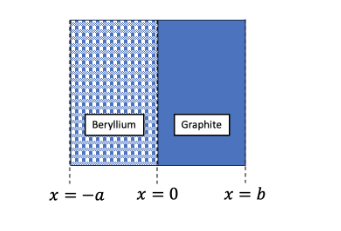
\includegraphics[width=0.4\linewidth]{figures/hw4Q_planes.png}
\end{figure}

\begin{enumerate}
\item[(a)] ({\bf 10 points}) Derive an expression for the neutron flux in the system.
\item[(b)] ({\bf 4 points}) Plot the flux for $D_1=0.1$ [cm], $D_2=0.8$ [cm], $L_1=1.0$ [cm], $L_2=7.0$ [cm], $a=20$ [cm], $b=30$ [cm], and $S=10^{10}$ [neutrons/s]. Region 1 is the beryllium, and region 2 is the graphite. Qualitatively describe the behavior.
\end{enumerate}


\clearpage
\noindent 6. ({\bf deep concept understanding}) For each of the following statements, indicate whether the statement is true or false. Provide an explanation.

\begin{enumerate}
\item[(a)] ({\bf 5 points}) (True/False) At a material interface between regions of different $\Sigma$, only some of the components of $\vec{J}$ are continuous across the interface.
\item[(b)] ({\bf 5 points}) (True/False) At a material interface, the gradient in flux must be continuous.
\item[(c)] ({\bf 5 points}) (True/False) When we write the diffusion equation as shown below, this means that neutrons only travel in the $\pm x$ directions.

\beq
-D\frac{d^2\phi}{dx^2}+\Sigma_a\phi=S
\eeq
\end{enumerate}


\end{document}

